%%% template.tex
%%%
%%% This LaTeX source document can be used as the basis for your technical
%%% paper or abstract. Intentionally stripped of annotation, the parameters
%%% and commands should be adjusted for your particular paper - title, 
%%% author, article DOI, etc.
%%% The accompanying ``template.annotated.tex'' provides copious annotation
%%% for the commands and parameters found in the source document. (The code
%%% is identical in ``template.tex'' and ``template.annotated.tex.'')

\documentclass[conference]{acmsiggraph}

\TOGonlineid{45678}
\TOGvolume{0}
\TOGnumber{0}
\TOGarticleDOI{1111111.2222222}
\TOGprojectURL{}
\TOGvideoURL{}
\TOGdataURL{}
\TOGcodeURL{}

\title{3D Printing for Mobile Robots}

\author{Andrew Spielberg\thanks{e-mail:aespielberg@csail.mit.edu} \and Vicki Crosson\thanks{e-mail:viccro.mit@gmail.com}}
\pdfauthor{Andrew Spielberg and Vicki Crosson}



\keywords{3D Printing, Robotics, 3Doodler, Trajectory Controller}

\begin{document}

%% \teaser{
%%   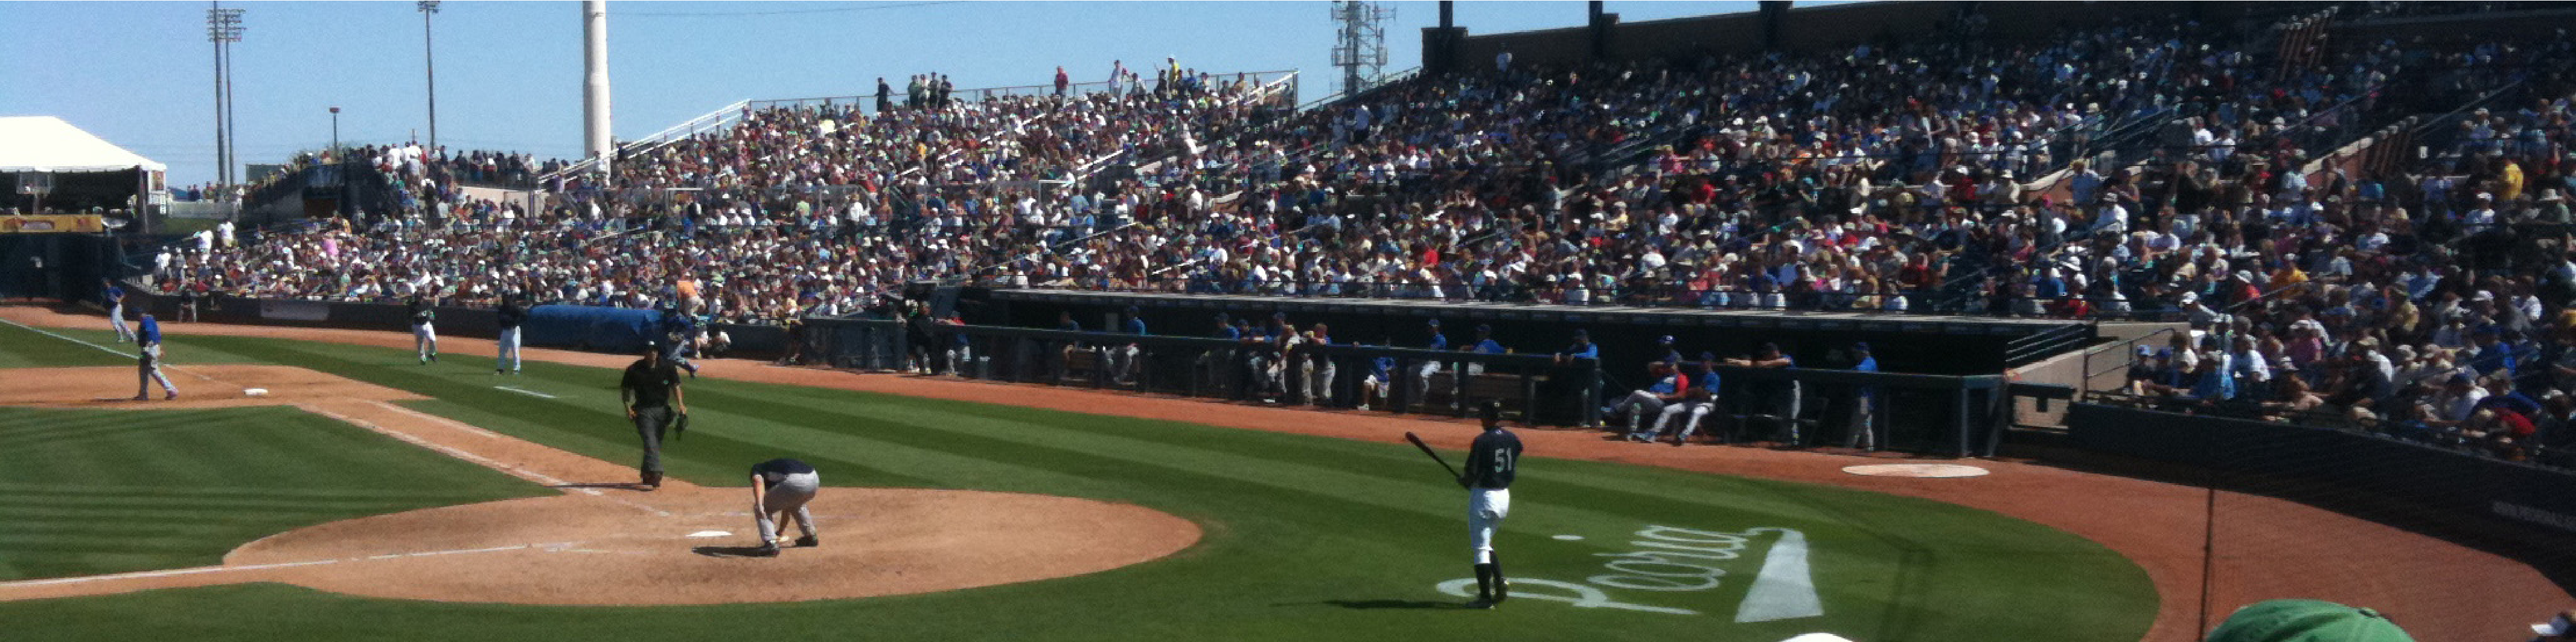
\includegraphics[height=1.5in]{images/sampleteaser}
%%   \caption{Spring Training 2009, Peoria, AZ.}
%% }

\maketitle

\begin{abstract}

Midway project report.

\end{abstract}

%\begin{CRcatlist}
%  \CRcat{I.3.3}{Computer Graphics}{Three-Dimensional %Graphics and Realism}{Display Algorithms}
%  \CRcat{I.3.7}{Computer Graphics}{Three-Dimensional %Graphics and Realism}{Radiosity};
%\end{CRcatlist}

\keywordlist

%% Use this only if you're preparing a technical paper to be published in the 
%% ACM 'Transactions on Graphics' journal.

\TOGlinkslist

%% Required for all content. 

\copyrightspace

\section{Introduction}

For our project, we seek to equip a Kuka YouBot (TODO: image) with a plastic extruder (namely, the 3Doodler) in order to allow a mobile manipulator to create freeform 3D shapes.  As the 3Doodler can only extrude plastic strands, all shapes that we create must be compositions of 3D curve segments.

Creating such a system requires several components, which we outline here.  In particular, the system requires:

\begin{itemize}
\item A tool for holding the 3Doodler in the youbot's fingers.
\item An electronics interface to the 3Doodler to allow it to be remotely controlled and monitored via the YouBot PC.
\item A GUI which allows users to easily create designs.
\item A tool for exporting those designs to an ordered collection of paths for the YouBot gripper to draw.
\item A velocity controller for the YouBot arm which allows for smooth extrusion in three dimensions without collisions upon previously extruded paths.
\end{itemize}

We now, in turn, discuss each of these components, their challenges, how they are currently being implemented, the remaining work which we'll aim to deliver in this class, and what will probably have to be left for future work.  Finally, we discuss our goal for our final deliverable (demonstration prints).

Our code is being hosted on Github in a private repository, if you would like access to see our files we can add you to the repository!



\section{YouBot 3Doodler Clamp Tool}


\section{Electronics for ROS-3Doodler Interfacing}
TODO: Vicki

\section{GUI}

\section{Path Ordering}

\section{YouBot controller and Path Planning}

\section{Demonstrations}
TODO: Vicki



\begin{figure}[ht]
  \centering
  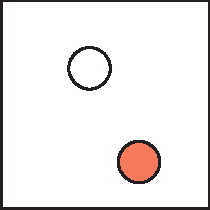
\includegraphics[width=1.5in]{images/samplefigure}
  \caption{Sample illustration.}
\end{figure}


\section{Exposition}



\section{Conclusion}




\bibliographystyle{acmsiggraph}
\bibliography{template}
\end{document}
